%% For double-blind review submission, w/o CCS and ACM Reference (max submission space)
\documentclass[sigplan,review,anonymous]{acmart}\settopmatter{printfolios=true,printccs=false,printacmref=false}
%% For double-blind review submission, w/ CCS and ACM Reference
%\documentclass[sigplan,review,anonymous]{acmart}\settopmatter{printfolios=true}
%% For single-blind review submission, w/o CCS and ACM Reference (max submission space)
%\documentclass[sigplan,review]{acmart}\settopmatter{printfolios=true,printccs=false,printacmref=false}
%% For single-blind review submission, w/ CCS and ACM Reference
%\documentclass[sigplan,review]{acmart}\settopmatter{printfolios=true}
%% For final camera-ready submission, w/ required CCS and ACM Reference
%\documentclass[sigplan]{acmart}\settopmatter{}


%% Conference information
%% Supplied to authors by publisher for camera-ready submission;
%% use defaults for review submission.
\acmConference[PL'18]{ACM SIGPLAN Conference on Programming Languages}{January 01--03, 2018}{New York, NY, USA}
\acmYear{2018}
\acmISBN{} % \acmISBN{978-x-xxxx-xxxx-x/YY/MM}
\acmDOI{} % \acmDOI{10.1145/nnnnnnn.nnnnnnn}
\startPage{1}

%% Copyright information
%% Supplied to authors (based on authors' rights management selection;
%% see authors.acm.org) by publisher for camera-ready submission;
%% use 'none' for review submission.
\setcopyright{none}
%\setcopyright{acmcopyright}
%\setcopyright{acmlicensed}
%\setcopyright{rightsretained}
%\copyrightyear{2018}           %% If different from \acmYear

%% Bibliography style
\bibliographystyle{ACM-Reference-Format}
%% Citation style
%\citestyle{acmauthoryear}  %% For author/year citations
%\citestyle{acmnumeric}     %% For numeric citations
%\setcitestyle{nosort}      %% With 'acmnumeric', to disable automatic
                            %% sorting of references within a single citation;
                            %% e.g., \cite{Smith99,Carpenter05,Baker12}
                            %% rendered as [14,5,2] rather than [2,5,14].
%\setcitesyle{nocompress}   %% With 'acmnumeric', to disable automatic
                            %% compression of sequential references within a
                            %% single citation;
                            %% e.g., \cite{Baker12,Baker14,Baker16}
                            %% rendered as [2,3,4] rather than [2-4].


%%%%%%%%%%%%%%%%%%%%%%%%%%%%%%%%%%%%%%%%%%%%%%%%%%%%%%%%%%%%%%%%%%%%%%
%% Note: Authors migrating a paper from traditional SIGPLAN
%% proceedings format to PACMPL format must update the
%% '\documentclass' and topmatter commands above; see
%% 'acmart-pacmpl-template.tex'.
%%%%%%%%%%%%%%%%%%%%%%%%%%%%%%%%%%%%%%%%%%%%%%%%%%%%%%%%%%%%%%%%%%%%%%


%% Some recommended packages.
\usepackage{booktabs}   %% For formal tables:
                        %% http://ctan.org/pkg/booktabs
\usepackage{subcaption} %% For complex figures with subfigures/subcaptions
                        %% http://ctan.org/pkg/subcaption

%%
\newcommand\question[1]{{\color{violet}#1}}
\newcommand\todo[1]{{\color{red}#1}}
%%

%%code things
\usepackage{listings}
\usepackage{xcolor}
 
\definecolor{codegreen}{rgb}{0,0.6,0}
\definecolor{codegray}{rgb}{0.5,0.5,0.5}
\definecolor{codepurple}{rgb}{0.58,0,0.82}
\definecolor{backcolour}{rgb}{0.97,0.97,0.97}

\lstdefinestyle{mystyle}{
    backgroundcolor=\color{backcolour},   
    commentstyle=\color{codegreen},
    keywordstyle=\color{magenta},
    numberstyle=\tiny\color{codegray},
    stringstyle=\color{codepurple},
    basicstyle=\ttfamily\footnotesize,
    breakatwhitespace=false,         
    breaklines=true,                 
    captionpos=b,                    
    keepspaces=true,                 
    numbers=left,                    
    numbersep=5pt,                  
    showspaces=false,                
    showstringspaces=false,
    showtabs=false,                  
    tabsize=2
}

\begin{document}

%% Title information
\title[Short Title]{\todo{Optimizing GPU Programs By Partial Evaluation}}         %% [Short Title] is optional;
                                        %% when present, will be used in
                                        %% header instead of Full Title.
\titlenote{with title note}             %% \titlenote is optional;
                                        %% can be repeated if necessary;
                                        %% contents suppressed with 'anonymous'
\subtitle{Subtitle}                     %% \subtitle is optional
\subtitlenote{with subtitle note}       %% \subtitlenote is optional;
                                        %% can be repeated if necessary;
                                        %% contents suppressed with 'anonymous'


%% Author information
%% Contents and number of authors suppressed with 'anonymous'.
%% Each author should be introduced by \author, followed by
%% \authornote (optional), \orcid (optional), \affiliation, and
%% \email.
%% An author may have multiple affiliations and/or emails; repeat the
%% appropriate command.
%% Many elements are not rendered, but should be provided for metadata
%% extraction tools.

%% Author with single affiliation.
\author{First1 Last1}
\authornote{with author1 note}          %% \authornote is optional;
                                        %% can be repeated if necessary
\orcid{nnnn-nnnn-nnnn-nnnn}             %% \orcid is optional
\affiliation{
  \position{Position1}
  \department{Department1}              %% \department is recommended
  \institution{Institution1}            %% \institution is required
  \streetaddress{Street1 Address1}
  \city{City1}
  \state{State1}
  \postcode{Post-Code1}
  \country{Country1}                    %% \country is recommended
}
\email{first1.last1@inst1.edu}          %% \email is recommended

%% Author with two affiliations and emails.
\author{First2 Last2}
\authornote{with author2 note}          %% \authornote is optional;
                                        %% can be repeated if necessary
\orcid{nnnn-nnnn-nnnn-nnnn}             %% \orcid is optional
\affiliation{
  \position{Position2a}
  \department{Department2a}             %% \department is recommended
  \institution{Institution2a}           %% \institution is required
  \streetaddress{Street2a Address2a}
  \city{City2a}
  \state{State2a}
  \postcode{Post-Code2a}
  \country{Country2a}                   %% \country is recommended
}
\email{first2.last2@inst2a.com}         %% \email is recommended
\affiliation{
  \position{Position2b}
  \department{Department2b}             %% \department is recommended
  \institution{Institution2b}           %% \institution is required
  \streetaddress{Street3b Address2b}
  \city{City2b}
  \state{State2b}
  \postcode{Post-Code2b}
  \country{Country2b}                   %% \country is recommended
}
\email{first2.last2@inst2b.org}         %% \email is recommended


%% Abstract
%% Note: \begin{abstract}...\end{abstract} environment must come
%% before \maketitle command
\begin{abstract}
GPUs have been known to be used to facilitate computation-\\ally-intensive problems solving.
And while this approach allows speed ups to the orders of magnitude, it is often challenging to achieve maximum performance. Also, while memory optimizations are being the most significant ones, GPUs memory hierarchy implies certain limitations, thus memory should be utilized carefully. Generally, on-chip data access is to be preferred over global one.
This paper proposes the idea of leveraging static\footnote{Compile-time known data or data that can be determined not to be changing during runtime} data memory management, using partial evaluation, a program transformation technique that enables the data to be embedded into the code and eventually end up directly in the registers. \question{Generalization to runtime detection of static?}
An empirical evaluation of a straightforward string pattern matching algorithm implementation \question{utilizing} this technique is provided.
\question{Our approach achieves up to $6x$\ performance gain compared to a straightforward naive CUDA C implementation.}  
\end{abstract}


%% 2012 ACM Computing Classification System (CSS) concepts
%% Generate at 'http://dl.acm.org/ccs/ccs.cfm'.
\begin{CCSXML}
<ccs2012>
<concept>
<concept_id>10011007.10011006.10011008</concept_id>
<concept_desc>Software and its engineering~General programming languages</concept_desc>
<concept_significance>500</concept_significance>
</concept>
<concept>
<concept_id>10003456.10003457.10003521.10003525</concept_id>
<concept_desc>Social and professional topics~History of programming languages</concept_desc>
<concept_significance>300</concept_significance>
</concept>
</ccs2012>
\end{CCSXML}

\ccsdesc[500]{Software and its engineering~General programming languages}
\ccsdesc[300]{Social and professional topics~History of programming languages}
%% End of generated code


%% Keywords
%% comma separated list
\keywords{GPU, CUDA, Partial Evaluation}  %% \keywords are mandatory in final camera-ready submission


%% \maketitle
%% Note: \maketitle command must come after title commands, author
%% commands, abstract environment, Computing Classification System
%% environment and commands, and keywords command.
\maketitle


\section{Introduction}

\todo{GPUs performance could be optimized via memory, instructions and configuration.} \question{Any statistics that memory optimizations are needed more often?}
\todo{However, with most applications tending to be bandwidth bound, memory optimizations appear to be in a prevailing significance.}
The GPUs memory access latency varies between different memory types, from hundreds of cycles for global memory to just a few for shared and register memory.
Moreover, the latency could be aggravated by wrong access patterns or misaligned accesses and the possibility of proper access patterns could depend on the domain of the problem being solved.
For example, global memory access \todo{order} could be not clear, thus preventing GPU from efficient coalescing. It imposes a burden of memory management to a programmer or make one to rely on caching mechanisms. 

In order to achieve the fastest memory access constant, shared or registers memory should be utilized.
However, constant memory lacks flexibility in a sense that the size of data should be known beforehand and access \todo{order} also should be kept in mind. Shared memory is to be used carefully due to considerations of synchronization and bank conflicts, while register allocation is managed by the compiler and explicit storing of data to them is difficult.
E.g. small arrays could be stored to registers, but only if the compiler is able to figure out that arrays indexing is static and if it does not, the array would end up in local memory.

\todo{Given that caches tend to undergo misses and random access could hurt coalescing or broadcasting}, we exploit partial evaluation techniques to specialize a GPU program on static data in such a way to move the data straight into the code rather than to any memory space.

\question{Partial evaluation is a program transformation optimization technique that emphasizes on full automation.\cite{Jones:1993:PEA:153676}
Basically, given a function $f$ of $n$ arguments with some of them being static, denoted with $k$, partial evaluator evaluates or \textit{specializes} those parts of the function depending only on static arguments, producing a residual function $f'$ of $(n-k)$ arguments.
Thus it gives a more optimal function in a sense that the function needs less computations when being actually invoked.}

Regarding GPU memory management partial evaluation is able to produce an optimization of memory access.
Consider the snippet of code from \hyperref[lst1]{\textbf{Listing 1}}.
Suppose the array named \textit{template} and its size \textit{template\_size} are statically known. The array \textit{ibuffer} is dynamic.
Given that memory access indexing and the content of the array are static, the snippet could be transformed to \textit{.ptx} instructions during the compilation as presented in \hyperref[lst2]{\textbf{Listing 2}}.
The thing is the content of \textit{template} array has been embedded into the comparison instructions rather than to be globally loaded multiple times as in \hyperref[lst2]{\textbf{Listing 3}}.  
\lstset{style=mystyle}
% \begin{figure}[b]
% \begin{lstlisting}[language=C,caption=Partial evaluation example,label=lst1]
% /*
% *   Suppose we have static template_size and
% *    template array itself, assume ['a',...] 
% */

%  for i in unroll(0,template_size) {
    % //global/constant memory access
    % if ibuffer(t_id + i as i64) != template(i) { 
        % //... Do something ... //
    % }
%  }
% /*
% *   After the specialization the code above        
% *    is transformed to an unrolled list of 
% *   akin .cu instructions
% */
    % ...
%  bool _93951;
%  _93951 = _93949 != 97; // 97 is ascii for 'a'
%  if (_93951) goto l93952;
%  else goto l93955;
    % ...
% \end{lstlisting}
% \end{figure}

% here are some silly things =)
% As long as the limitation on the number of registers per thread is met, all static data eventually \todo{get} into registers memory.
% \question{Moreover, if excessive usage of register memory happens, data would automatically leak to cached local memory resulting in automatic memory management, i.e. avoiding explicit allocations.}

\begin{figure}[b]
\begin{lstlisting}[language=C,caption=Partial evaluation example,label=lst1]
/*
*   assume  template is ['\x49','\x44',...]  
*/

 for i in unroll(0,template_size) {
    //global/constant memory access
    if ibuffer(t_id + i as i64) != template(i) { 
        //... Do something ... //
    }
 }
\end{lstlisting}
\end{figure}

\begin{figure}[b]
\begin{lstlisting}[language=C,caption=Code after partial evaluation,label=lst2]
    ...
 LDG.E.U8 R0, [R4] ; //load from global memory, i.e. ibuffer(...)
 BFE R6, R0, 0x1000 ;
 ISETP.NE.AND P0, PT, R6, 0x49, PT ; //0x49 got extracted, so we have avoided global memory access!
 @P0 SYNC ;
 LDG.E.U8 R0, [R4+0x1] ;
 BFE R0, R0, 0x1000 ;
 ISETP.NE.AND P0, PT, R0, 0x44, PT ; //extracted again!
    //and so on
    ...
\end{lstlisting}
\end{figure}

\begin{figure}[b]
\begin{lstlisting}[language=C,caption=Code without partial evaluation,label=lst3]
 LDG.E.U8 R8, [R8] //load global
 LDG.E.U8 R6, [R6] ; // load global
 BFE R13, R8, 0x1000 ;
 BFE R12, R6, 0x1000 ;
 ISETP.NE.AND P0, PT, R13, R12, PT ; //compare pre-loaded registers

\end{lstlisting}
\end{figure}

The partial evaluator being used is one developed as part of \textit{AnyDSL} framework.
\question{The specialized achieves got up to $6x$ better performance compared to straightforward implementations with \textit{CUDA C}.}

\begin{figure}[ht]
\centering
    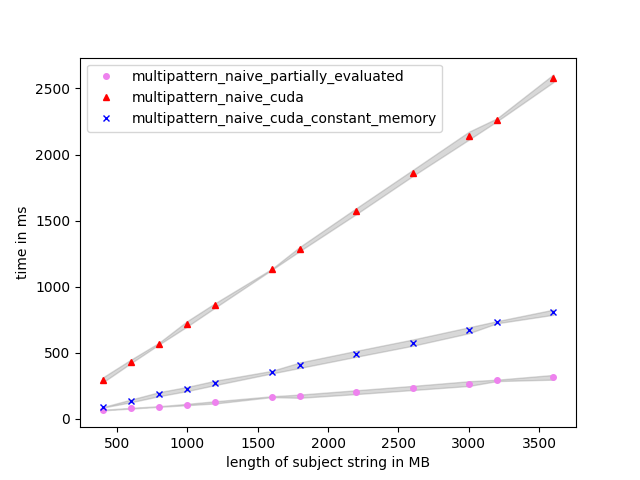
\includegraphics[scale=0.5]{results_multipattern_final.png}
    \caption{Multiple string pattern matching evaluation.}
    \label{fig:eval}
\end{figure}

\section{Performance Evaluation}
The approach has been evaluated on Ubuntu 18.04 system with \textit{Intel Core i7-6700} processor, 8GB of RAM and \textit{Pascal}-based \textit{GeForce GTX 1070} GPU with 8GB device memory.

To estimate the performance gain brought by partial evaluation the problem of searching multiple string occurrences in some subject string has been considered.
The problem arises in many areas like computer security or bioinformatics where the patterns are often known beforehand, rather small and to be searched in huge arrays of data. 

For the evaluation the piece of data of 4 GB size has been taken from a hard drive and patterns to be searched have been taken from a taxonomy of file headers specifications.
The patterns have been divided to groups of size 16 and run over multiple times. The results are presented in \hyperref[fig:eval]{\textbf{Figure 1}}.
The points are the average kernel running time and the gray regions are the area of standard deviation.   

The evaluation compares AnyDSL framework implementation leveraging partial evaluation with respect to the patterns against two base-line implementations in CUDA C with global and constant memory for patterns storing respectively. 
All implementations invoke the algorithm in a separate thread for each position in the subject string.

The patterns are stored as a single char-array and accessed via offsets.
The algorithm simply iterates over all patterns searching for a match, if it encounters a mismatch, it jumps to the next pattern forward through the array.
Since the patterns could be lengthy and mismatches happen quite often, such access pattern hurts coalescing, increasing the overall number of memory transactions. 
Given that, the performance speed up partially evaluated algorithm achieves is up to $6x$  compared to CUDA C version with global memory and up to $3x$ with constant one as illustrated in \hyperref[fig:eval]{\textbf{Figure 1}}. 

\section{Conclusion}
The work proposes the idea of applying partial evaluation to optimize GPU programs. The program transformation moves data from arrays directly into the code, thus enhancing performance due to memory access transactions number reduction. \todo{It results in a noticeable performance gain but not always.}
    
The partial evaluator being used assumes the programs to be written with special \textit{DSL} and up to the current level of progress requires the array-like data to be passed \todo{inplace} for \textit{JIT} compiler to be able to extract information from it. \question{+ maybe add a remark that PE could enhance programs asymptotically}. Nevertheless, this could be \todo{rectified} with \todo{symbolic computation?} and we strongly believe that GPU specialization is \question{possible in runtime, i.e. during kernel execution}.

%% Acknowledgments
\begin{acks}                            %% acks environment is optional
                                        %% contents suppressed with 'anonymous'
  %% Commands \grantsponsor{<sponsorID>}{<name>}{<url>} and
  %% \grantnum[<url>]{<sponsorID>}{<number>} should be used to
  %% acknowledge financial support and will be used by metadata
  %% extraction tools.
  This material is based upon work supported by the
  \grantsponsor{GS100000001}{National Science
    Foundation}{http://dx.doi.org/10.13039/100000001} under Grant
  No.~\grantnum{GS100000001}{nnnnnnn} and Grant
  No.~\grantnum{GS100000001}{mmmmmmm}.  Any opinions, findings, and
  conclusions or recommendations expressed in this material are those
  of the author and do not necessarily reflect the views of the
  National Science Foundation.
\end{acks}


%% Bibliography
\bibliography{bib.bib}


%% Appendix
% \appendix
% \section{Appendix}

% Text of appendix \ldots

\end{document}
